\documentclass[12pt]{article}
\usepackage[a4paper, left = 35mm, top = 24mm, bottom = 24mm, right = 24mm]{geometry}
\usepackage{amsfonts, amsmath, amssymb}
\usepackage{gensymb}
\usepackage{fancyhdr}
\usepackage{pdfpages}
\usepackage{listings}
\usepackage{color}
\usepackage{pdfpages}
\usepackage{hyperref}
\usepackage{verbatim}
\usepackage[utf8]{inputenc}
\usepackage{graphicx}
\usepackage{float}
\usepackage{longtable}
\usepackage{fontenc}
\usepackage[backend=biber, style=ieee]{biblatex}
\usepackage{fontenc}
\usepackage{times}
\usepackage[ddmmyyyy]{datetime}
\usepackage{pdfpages}
\usepackage{subcaption}
\usepackage{multirow}
\usepackage{epstopdf}
\usepackage{dirtree}
\usepackage{listings}

\addbibresource{biblo.bib}

%To make captions centered and italic
\usepackage[format=plain, labelfont=bf, textfont=it, justification=centering]{caption}
%To add custom indents to bullet points
\usepackage{enumitem}


\pagestyle{empty}

\setlength{\parindent}{0pt}
\setlength{\parskip}{1em}

\makeatletter
\newcommand*{\rom}[1]{\expandafter\@slowromancap\romannumeral #1@} %Allows a call of \rom{*NUM*} to output the roman numeral of NUM 
\makeatother

%New colors defined below
\definecolor{codegreen}{rgb}{0,0.6,0}
\definecolor{codegray}{rgb}{0.5,0.5,0.5}
\definecolor{codepurple}{rgb}{0.58,0,0.82}
\definecolor{backcolour}{rgb}{0.95,0.95,0.92}

%Code listing style named "mystyle"
\lstdefinestyle{mystyle}{
  backgroundcolor=\color{backcolour},   commentstyle=\color{codegreen},
  keywordstyle=\color{magenta},
  numberstyle=\tiny\color{codegray},
  stringstyle=\color{codepurple},
  basicstyle=\ttfamily\scriptsize,
  breakatwhitespace=false,         
  breaklines=true,                 
  captionpos=b,                    
  keepspaces=true,                 
  numbers=left,                    
  numbersep=5pt,                  
  showspaces=false,                
  showstringspaces=false,
  showtabs=false,                  
  tabsize=2
}

%"mystyle" code listing set
\lstset{style=mystyle}

\begin{document}
%TC:ignore
\begin{titlepage}
    \newgeometry{left=4cm, right=4cm, top=4cm, bottom=4cm}
    \begin{center}
        {\LARGE Electronics and Computer Science\\ Faculty of Engineering and Physical Sciences\\}
        \vspace{0.4cm}
        {\LARGE University of Southampton}
        
        \vfill
        % Authors
        {\Large Peter Alexander\\}
        
        \vspace{1cm}
        {\Large \today\\}
        \vspace{1cm}
        % Title
        {\LARGE COMP6202: Evolution of Complexity\\}
        {\Large Assignment 2\\}
        \vfill
        %Supervisors
        {\Large Module Leader: Richard Watson\\}
        \vspace{0.3cm}
        {\Large Moderator: Danesh Tarapore\\}
        \vfill
        \Large A Report submitted for the Award of MEng Electronic Engineering

    \end{center}
    \restoregeometry
\end{titlepage}
%TC:endignore

\section*{Abstract}
\newpage


\newpage
\setcounter{tocdepth}{2}

%TC:ignore
\newpage
\tableofcontents
\newpage
%TC:endignore
\setcounter{page}{1}
\pagestyle{plain}

% Include PDFs of content Here %
%------------------------------%
\section{Introduction} \label{sec:introduction}

The third paper, \textit{A Cooperative Coevolutionary Approach to Function Optimisation}\cite{original-paper} was chosen for this assignment.
The paper presents a framework for a Cooperative Coevolutionary Genetic Algorithm (CCGA) and compares its performance with a standard Genetic Algorithm (GA) in function optimisation problem.

The functions were chosen for being \textit{``highly multi-modal''}, presenting a difficult challenge for a hill-climber.
These functions are referred to as the Rastrigin, Schwefel, Griewangk, and Ackley functions\cite{functions-1,functions-2,functions-3}.
Each of these functions has a global minimum of zero when the set of parameters fed into it are bounded by set values.
The optimisation task presented in the paper is to evolve the set of parameters that give an output of zero.
Each algorithm's performance is tested on each function individually.

In the standard GA, the individuals being evolved are bit-strings representing every parameter.
The fitness of each individual is calculated by by splitting the bit-string into the parameters and running it through the function.
In the CCGA, each parameter is represented by its own population of bit-strings.
Each population is evaluated in a round-robin fashion.
The fitness of each individual is calculated by combining it with the best individuals from each of the other populations and running this set through the function.
An initial fitness value is assigned before the first generation by evaluating each individual with a random individual from each population.
In both algorithms, the closer the function output is to zero, the fitter the individual.

A scaling window is used to translate this smaller-is-better fitness regime into a fitness proportionate selection scheme.
When calculating the selection probability of an individual its fitness is subtracted from the fitness of the worst individual from the past 5 generations.
This value is used when calculating the size of an individuals 'slice' on the roulette wheel.
This also allows small variations in the population to standout relative to the rest of the population.

Table \ref{tab:parameter-table}, reproduced from the original paper, contains the algorithm characteristics used in the experiments.


\begin{table} [h]
    \begin{tabular}{|l|l|}
        \hline
        \textbf{Characteristic}      & \textbf{Value}                       \\
        \hline
        Representation          & Binary (16 bits per function parameter)   \\
        Selection               & Fitness Proportionate                     \\
        Fitness Scaling         & Scaling Window Technique (width 5)        \\
        Elitist Strategy        & Single copy of best individual preserved  \\
        Genetic Operators       & Two-point crossover and bit-flip mutation \\
        Mutation Probability    & 1/chromlength                             \\
        Crossover Probability   & 0.6                                       \\
        Population Size         & 100                                       \\
        Simulation Length       & 100000 function evaluations               \\
        \hline

    \end{tabular}
    \caption{A table showing the characteristics of the algorithms used to perform the experiments. Reproduced from \cite{original-paper}}
    \label{tab:parameter-table}
\end{table}

\section{Reimplementation} \label{sec:reimplementation}

The reimplementation was written in Python v3.8 for flexibility and speed of development.
The results generated by the Python script were saved to disk and plotted using MATLAB.
This meant plots could be fine tuned without having to rerun the experiments.

Individuals are defined using an \texttt{Individual} class in \texttt{individual.py} (Appendix \ref{lst:individual}). 
This class defines the genome as a BitArray object (defined in the third-party bistring library\cite{bistring-repo}), and that individual's fitness for convenience.
The fitness functions are defined in \texttt{functions.py} (Appendix \ref{lst:functions}). 
Each function is defined with identical interfaces and an accompanying Python dict containing details about the function such as the limits of the parameter values.
Also included are functions to convert a set of BitArrays to function parameters.
The original paper did not specify the conversion process used so the range of $[0, 2^{16} - 1]$ that the BitArray can represent is mapped to the lower and upper limits of the functions (e.g. $[-5.12, 5.12]$ for the Rastrigin function).

The algorithms are implemented in the classes \texttt{GAExperiment} and \texttt{CCGAExperiment} (see Appendices \ref{lst:ga_experiment}, \ref{lst:ccga_experiment}). 
These classes implement generic versions of their algorithm and must be provided with the fitness function, the corresponding Python dict, and the number of parameters under test upon instantiation.
The experiment can then be run using the \texttt{run\_experiment()} method.
The \texttt{CCGAExperiment} class shares the same overall structure as the \texttt{GAExperiment} class but has been upgraded with the infrastructure needed to store, evolve, and evaluate multiple populations.

The experiments are performed in the file \texttt{main\_data\_gather.py} (see Appendix \ref{lst:main_data_gather}).
This acts as the project's main file.
The user specifies which algorithms should be tested and the number of runs the results should be averaged over with command line arguments.
The results are saved to txt files for plotting.
The computing resources available to this project were limited due to working from home so results of each experiment were averaged over 15 runs rather than the 50 in the original paper.

The MATLAB script \texttt{combined\_plots.m} (see Appendix \ref{lst:combined_plots}) was used to produce the reimplemented figure.

\section{Reimplementation Results} \label{sec:reimplementation-results}

Figure \ref{fig:original_plot} shows the results from the original paper and Figure \ref{fig:combined_plot} shows the reimplementation results.
It can be seen that both plots show the same trajectory for the fitness over the series of function evaluations.
The reimplementation plots show slightly rougher due to the lower number of experiments used to calculate the average performance. 

\begin{figure}[ht!]
    \centering 
    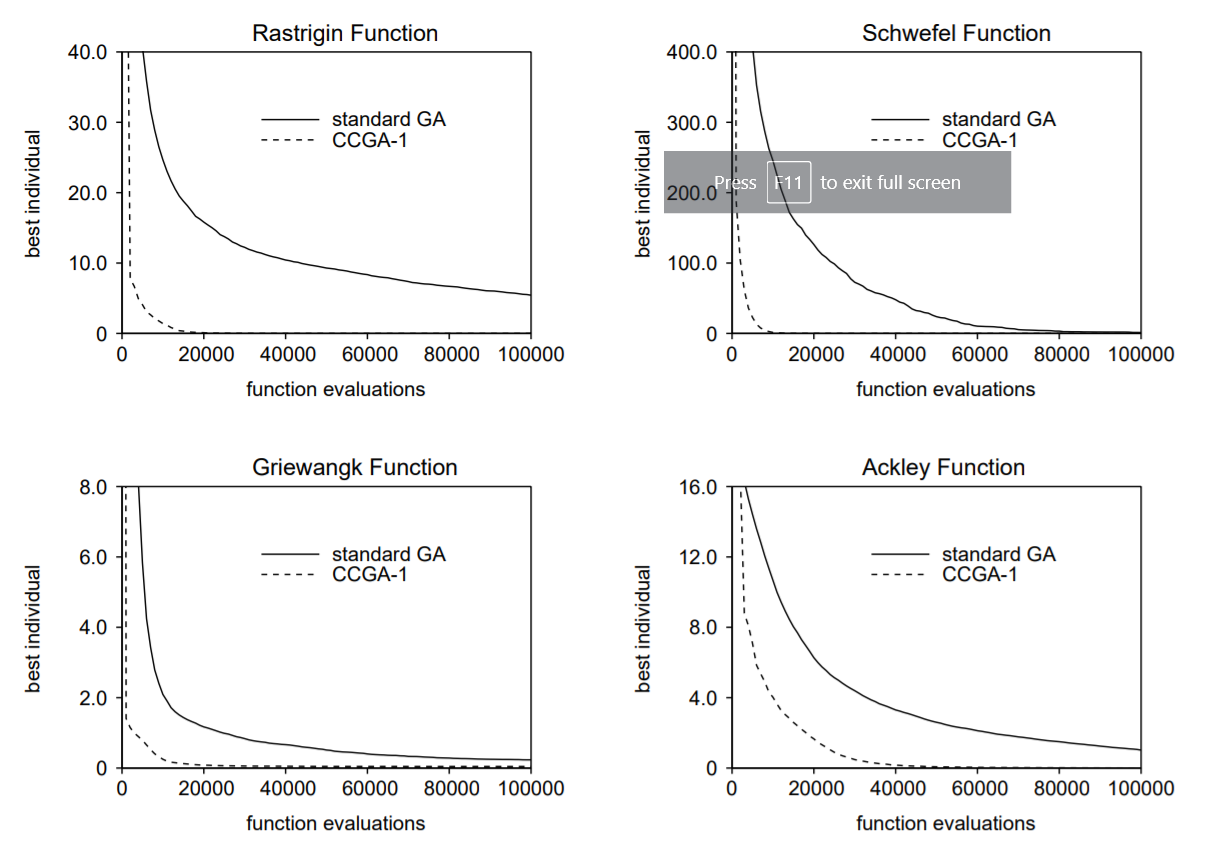
\includegraphics[width=0.9\textwidth]{img/original_plot.png}
    \caption{The figure this assignment aims to reimplement. Reproduced from\cite{original-paper}.}
    \label{fig:original_plot}
  \end{figure}

  \begin{figure}[ht!]
    \centering 
    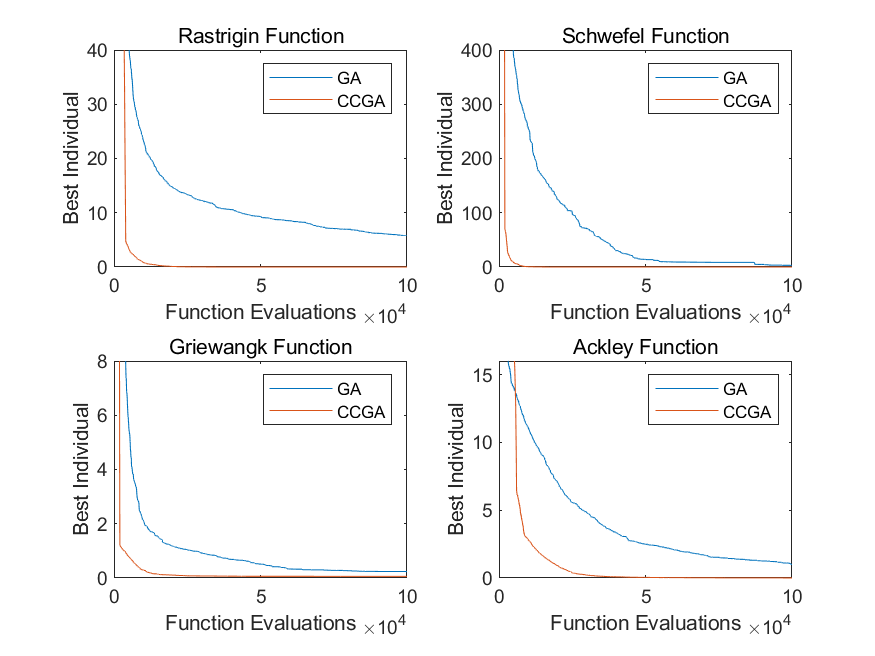
\includegraphics[width=0.9\textwidth]{img/combined_plot.png}
    \caption{The figure produced by this reimplementation.}
    \label{fig:combined_plot}
  \end{figure}

\section{Extension} \label{sec:extension}

When reading the original paper and surrounding literature it was noted that while of the characteristics given in Table \ref{tab:parameter-table} impact each algorithm equally, there is one area where it seems the CCGA has an unfair advantage.
By performing a two point crossover on each individual in the CCGA it is effectively performing an N point crossover on the problem as a whole. 
Whilst the number of crossovers does not change between the two algorithms as the number of fitness evaluations are fixed, it still enables evolution to occur at a more granular level in the CCGA.
It is thought that these properties have a small but measurable impact on the CCGA's peprformance, but the majority comes from how fitness data is measured and stored.


The hypothesis that is presented in this extension is as follows:

\emph{The performance increase of the CCGA over the standard GA comes from the ability to effectively measure the fitness of individual genes rather than entire genomes, not the more granular crossover scheme a CCGA enables.} 

Where \textit{gene} refers to a 16 bit chunk that encodes a single function parameter.
To test this, two new crossover functions were added to the GA:
\begin{enumerate}
    \item \textbf{N Point/Chunk Crossover} - In this scheme, two parents are selected as is the case for two point crossover. However, rather than combining two contiguous halves from each parent to produce the offspring, each 16-bit chunk is taken from a randomly selected parent. 
    This can be thought of like N chunk uniform crossover.
    This accounts for the situation where both parents have good and bad genes distributed throughout rather than just in one half.

    \item \textbf{N Individual Crossover} -  This is an extension of the scheme above.
    Here each individual has a number of parents equal to the number of function parameters.
    Like before, each 16-bit chunk is taken from a randomly selected parent.
    This means that each function evaluation is able to sample a wider range of the population.
    This crossover method is combined with standard two point crossover to allow genes to be split occasionally.
\end{enumerate}

Both these schemes aim to equalise the playing field between the GA and the CCGA where crossover is concerned.
They constitute reasonable drop-in improvements to a standard GA that aim to mimic the granularity of a CCGA without adding the infrastructure needed for multiple populations.
The two schemes shall be referred to as the EXGA\_1 and the EXGA\_2.

A plot showing the results of this extension was produced by the MATLAB script \\
\texttt{extension\_plot.m} (see Appendix \ref{lst:extension_plots}).

\section{Extension Results} \label{sec:extension-results}

\section{Conclusion} \label{sec:conclusion}


\printbibliography

\pagestyle{empty}

\appendix

% Include PDFs of appendices here %
%TC:ignore
\section{Source Code Listing} \label{sec:source-code-listing}

\lstlistoflistings

\subsection{individual.py} \label{lst:individual}
\lstinputlisting[language=Python,caption=individual.py]{../Implementation/src/individual.py}

\subsection{functions.py} \label{lst:functions}
\lstinputlisting[language=Python,caption=functions.py]{../Implementation/src/functions.py}

\subsection{ga\_experiments.py} \label{lst:ga_experiment}
\lstinputlisting[language=Python,lastline=326,caption=ga\_experiment.py]{../Implementation/src/ga_experiment.py}

\subsection{ccga\_experiments.py} \label{lst:ccga_experiment}
\lstinputlisting[language=Python,lastline=329,caption=ccga\_experiment.py]{../Implementation/src/ccga_experiment.py}

\subsection{main\_data\_gather.py} \label{lst:main_data_gather}
\lstinputlisting[language=Python,caption=main\_data\_gather.py]{../Implementation/src/main_data_gather.py}

\subsection{combined\_plots.m} \label{lst:combined_plots}
\lstinputlisting[language=Matlab,caption=combined\_plots.py]{../Implementation/collected_data/matlab_plotting_scripts/combined_plots.m}

\subsection{extension\_plots.m} \label{lst:extension_plots}
\lstinputlisting[language=Matlab,caption=extension\_plots.py]{../Implementation/collected_data/matlab_plotting_scripts/extension_plots.m}

%TC:endignore
% ------------------------------- %

\end{document}